\def\ReportNumber{2}
\def\ReportName{Electrodynamic analysis}
\documentclass[11pt,a4paper]{article}
\usepackage[T1]{fontenc}
\usepackage[utf8]{inputenc}
\usepackage{newtxtext,newtxmath,microtype}
\usepackage[margin=21mm,headheight=14pt]{geometry}
\usepackage{booktabs,tabularx,array,amsmath,graphicx,float,caption}
\usepackage{xcolor,fancyhdr,lastpage,listings}
\usepackage[hidelinks]{hyperref}
\definecolor{accent}{HTML}{254C58}
% Original question wording: NMES Assignment 2026, Sections 1--3.
% Line-wrap hyphenation is removed; mathematical notation is typeset in LaTeX.
\usepackage{tcolorbox}
\newcommand{\assignmentquestion}[1]{%
  \begin{tcolorbox}[colback=accent!4,colframe=accent!65,
    boxrule=0.4pt,leftrule=2pt,arc=0pt,boxsep=0pt,
    left=7pt,right=7pt,top=5pt,bottom=5pt,
    before skip=0pt,after skip=8pt,fontupper=\small]
  \textbf{Assignment question.} #1
  \end{tcolorbox}%
}
\newcommand{\questionfiles}[1]{%
  \par\smallskip{\footnotesize\color{accent}
  \textbf{Files / results (relative to Source-code).} #1\par}\medskip
}
\newcommand{\QuestionOneOne}{%
Describe your cable: construction, dimensions, materials, rated voltage, rated
current (ampacity) and the laying conditions for which that rating is given
(burial depth, soil thermal resistivity, ambient temperature, arrangement).
Give a table of electromagnetic and thermal properties with a source for each value.}
\newcommand{\QuestionOneTwo}{%
Choose the environment consistently with the datasheet rating conditions,
and justify its properties.}
\newcommand{\QuestionOneThree}{%
State the sheath bonding you assume: single-point bonded (no net sheath current)
or solidly bonded (circulating sheath currents allowed), and how the armour
and pipe are connected. This choice strongly affects the losses in Section 3.}
\newcommand{\QuestionOneFour}{%
State the excitation you impose: phase-to-ground voltage and phase current,
as peak phasors, with the phase sequence (see the conventions in Appendix A).}
\newcommand{\QuestionTwoOne}{%
Define your computational domain, the equations solved and the boundary
conditions. Where do you truncate the domain, and why? Discuss the role of
the grounded screens: which regions actually influence the field in the insulation?}
\newcommand{\QuestionTwoTwo}{%
Can you simplify the geometry of your cable without degrading the precision
(e.g. disregard details in the geometrical description)? Quantify the effect
of each simplification.}
\newcommand{\QuestionTwoThree}{%
How do the results vary with the mesh refinement? Plot the maximum field in
the insulation and the capacitance versus the number of degrees of freedom,
and identify where local refinement is needed.}
\newcommand{\QuestionTwoFour}{%
Define the admissible field strength at the conductor screen and at the core
screen from the datasheet (or, if absent, from a cited reference).
Is the healthy cable within these limits?}
\newcommand{\QuestionTwoFive}{%
Add a defect to the insulation of your cable. State its nature (e.g. gas void,
water tree, protrusion of the semiconducting screen), its properties, size and
position, and discuss what a defect in a 2D cross-section represents in 3D.
Compare the field with and without defect along a radial cut.
Does the cable withstand the defect?}
\newcommand{\QuestionTwoSix}{%
Compute the resistive and displacement current densities in the cable.
Is current conservation satisfied? Which current dominates in each material, and why?}
\newcommand{\QuestionTwoSeven}{%
Compute the per-unit-length capacitance (\(\mu\mathrm{F/km}\)) and compare with
the analytical value (13) and with the datasheet. State the assumptions of the
analytical formula (in particular, how the semiconducting layers are treated).
Does the capacitance vary with frequency? Why (not)?}
\newcommand{\QuestionTwoEight}{%
Propose an improvement of the cable design with respect to the electric stress,
and support it quantitatively.}
\newcommand{\QuestionThreeOne}{%
Define your computational domain, the equations solved and the boundary conditions.
Where do you truncate the domain, and why? How do you impose the currents in the phase conductors?}
\newcommand{\QuestionThreeTwo}{%
\textbf{Conductor model.} Compare the skin depth in the conductor with its radius.
Model the phase conductors (a) as stranded conductors (imposed uniform current density)
and (b) as massive conductors (imposed net current, eddy currents allowed).
Which assumption is more realistic for your cable, and how does it affect the results?}
\newcommand{\QuestionThreeThree}{%
\textbf{Bonding.} Implement the bonding assumed in Q1.3 with global quantities
(net current and voltage per unit length in the sheaths, armour and pipe).
Explain why using only \(\mathbf j=-\mathrm i\omega\sigma\mathbf a\)
in these regions does not correspond to a well-defined bonding condition.}
\newcommand{\QuestionThreeFour}{%
Can you simplify the geometry without degrading the precision?
Are the simplifications of Section 2 still valid here?}
\newcommand{\QuestionThreeFive}{%
Check the mesh quality and refine where needed (element size compared with the
skin depth in each conducting region). How do losses, resistance and inductance
vary with the mesh refinement?}
\newcommand{\QuestionThreeSix}{%
Get the magnetic flux density (or induction) in and around your cable.}
\newcommand{\QuestionThreeSeven}{%
Get the current density in the conducting parts of your cable.}
\newcommand{\QuestionThreeEight}{%
Get the time-averaged Joule losses (kW/km) in each conducting part
(conductors, sheaths, armour, pipe, environment).}
\newcommand{\QuestionThreeNine}{%
Get the per-unit-length AC resistance (\(\Omega/\mathrm{km}\)), defined from
the total losses. Compare it with the DC resistance and with the datasheet.
Separate the contributions of skin/proximity effect and of sheath/armour losses.}
\newcommand{\QuestionThreeTen}{%
Get the per-unit-length inductance (mH/km). How do you define it for a
three-phase system? Does it vary with frequency? Compare with the datasheet.}
\newcommand{\QuestionThreeEleven}{%
Propose a design change that reduces the losses, and support it quantitatively.}

\pagestyle{fancy}\fancyhf{}
\fancyhead[L]{\small FE for Electromagnetic Fields -- Kutikuppala, Lefebure, Miseur}
\fancyhead[R]{\small NKT 33 kV, 185 + 50 mm\textsuperscript{2}}
\fancyfoot[L]{\small Section \ReportNumber\ -- \ReportName}
\fancyfoot[R]{\small\thepage\,/\,\pageref{LastPage}}
\renewcommand{\headrulewidth}{0.3pt}
\setlength{\parindent}{0pt}\setlength{\parskip}{5pt}
\setlength{\emergencystretch}{2em}
\setlength{\tabcolsep}{5pt}\renewcommand{\arraystretch}{1.13}
\captionsetup{font=small,labelfont=bf,skip=5pt}
\newcolumntype{Y}{>{\raggedright\arraybackslash}X}
\newcommand{\file}[1]{\href{../Source-code/#1}{\nolinkurl{#1}}}
\newcommand{\setupfile}[1]{\file{Cable-selection-and-model-setup/#1}}
\newcommand{\efile}{\file{Electrodynamic-analysis/cable.pro}}
\newcommand{\mfile}{\file{Magnetothermal-analysis/cable.pro}}
\newcommand{\runall}{\href{../run_all.sh}{\nolinkurl{run_all.sh}}}
\newcommand{\runE}{\texttt{getdp cable.pro -msh}\ \path{../Cable-selection-and-model-setup/cable.msh}\ \texttt{-solve Electrodynamics}}
\newcommand{\codeguide}[3]{\par\smallskip
 {\small\bfseries\color{accent}Code guide}\par\nobreak
 \begingroup\small\setlength{\tabcolsep}{0pt}
 \begin{tabularx}{\linewidth}{@{}p{14mm}Y@{}}
 \textbf{Files} & #1\\[2pt]
 \textbf{Run} & #2\\[2pt]
 \textbf{Check} & #3
 \end{tabularx}\par\endgroup\medskip}
\newcommand{\pending}{\textbf{Status: implementation still required.} }
\newcommand{\refurl}[2]{\href{#1}{#2}}
\lstset{basicstyle=\small\ttfamily,columns=fullflexible,keepspaces=true,
 showstringspaces=false,breaklines=true,upquote=true,
 backgroundcolor=\color{accent!4},frame=none,
 xleftmargin=5pt,xrightmargin=5pt,aboveskip=5pt,belowskip=5pt}
\hypersetup{pdftitle={Section \ReportNumber: \ReportName},
  pdfauthor={Kutikuppala Jaswanth, Lefebure Tiebert, Miseur Torre}}

\begin{document}
\section*{Q2.1 Domain, equations and boundaries}
\assignmentquestion{\QuestionTwoOne}
The active problem solves the three XLPE annuli, each between
\(r_i=7.8~\mathrm{mm}\) and \(r_o=15.8~\mathrm{mm}\). Both semiconducting
layers are treated as perfect equipotentials: the inner interface follows
its conductor voltage and the outer interface is grounded. The aluminium,
copper, fillers, jackets and soil are meshed but have no electric unknowns.
A blank field map in those regions is therefore expected.

\textbf{Equation.} With peak phasors and \(e^{j\omega t}\),
\[
 \hat{\mathbf E}=-\nabla\hat v,\qquad
 \nabla\!\cdot\big[(\sigma+j\omega\varepsilon)\hat{\mathbf E}\big]=0,
 \qquad \varepsilon=\varepsilon_0(2.5),\quad \sigma=10^{-18}~\mathrm{S/m}.
\]
Each region is homogeneous and isotropic, properties are independent of
frequency and temperature, and the cable is uniform and infinitely long in
the axial direction. End effects, terminations, dielectric dispersion and
partial discharge are omitted. Linear nodal triangles approximate the potential.

\textbf{Dirichlet conditions.} At the inner XLPE boundary, apply
\(26.9444~\mathrm{kV}\) peak at angles \(0,-120^\circ,+120^\circ\).
At each outer XLPE boundary, apply \(\hat v=0\). These boundaries are physical
groups 101/102/103 and 110, respectively.

The weak form used in \texttt{cable.pro} is, for test functions vanishing on
the voltage boundaries,
\[
 \int_{\Omega_{\rm XLPE}}(\sigma+j\omega\varepsilon)
       \nabla\hat v\cdot\nabla w\,dA=0.
\]
The \texttt{sigma} Galerkin term and the \texttt{DtDof[epsilon...]} term
implement conduction and displacement current, respectively.

\textbf{Truncation and shielding.} The electric domain ends at each grounded
outer XLPE interface. A 0.6 m square soil region is retained in the shared mesh
for later use, but no electric condition is applied there because it is outside
the solved domain. With ideal continuous grounded screens, the exterior and
neighbouring cable arrangement cannot change the internal electric solution.
This conclusion depends on the imposed screens; it does not cover a broken,
floating or resistive screen, or cable ends.

\codeguide{\efile: \texttt{Domain\_Ele}, \texttt{Constraint},
\texttt{Formulation} and \texttt{Resolution}.
\setupfile{cable.geo}: physical groups.
\file{Electrodynamic-analysis/cable.geo}: one-line entry to that shared geometry.}
{In Gmsh use \textbf{File > Open} on \efile, then press \textbf{Run}.
Keep \textbf{Jacket gap [mm]} at 0.5 for the baseline and use resolution
\texttt{Electrodynamics} with compute command \texttt{-solve}.}
{Open \texttt{res/potential.pos} and \texttt{res/field\_norm.pos} in Gmsh.
Only XLPE regions 41/42/43 should show fields. The 350 A axial load is not applied here.}

\newpage
\section*{Q2.2 Geometric simplifications}
\assignmentquestion{\QuestionTwoTwo}
With both XLPE interface potentials prescribed, each annulus solves a separate
boundary-value problem. Translating the cable leaves its radii, dielectric
properties and boundary voltages the same. Thus the exact solution for the
model gives identical peak field and capacitance at 0 and 0.5 mm gap. The
aluminium interior, copper wires and exterior soil can also be simplified
outside these ideal boundaries.

Screen thicknesses still determine the dielectric radii. Putting the inner
voltage at 7.4 rather than 7.8 mm would give
\(C'=0.18336~\mu\mathrm{F/km}\), 6.94\% lower. Finite screen conductivity
and surface roughness have not been checked against a detailed model.

\textbf{Paired FE check.} Both cases use 33 kV line-to-line RMS, 50 Hz,
8 mm XLPE and the same mesh controls. Only \texttt{JacketGap} changes.

\begin{center}\small
\begin{tabular}{@{}rrrr@{}}\toprule
Target \(h\) [mm] & Jacket gap [mm] & Peak \(E\) [kV/mm] & \(C'\) [\(\mu\)F/km]\\\midrule
0.250 & 0.0 & 4.87222 & 0.197032089\\
0.250 & 0.5 & 4.87288 & 0.197032070\\
0.125 & 0.0 & 4.88439 & 0.197030777\\
0.125 & 0.5 & 4.88622 & 0.197030777\\\bottomrule
\end{tabular}
\end{center}
Relative to touching, the gap raises the sampled peak by 0.0135\% at the
default size and 0.0375\% on the finer mesh. The capacitance differs by less
than 0.00001\% at either size. These small differences come from separately
generated triangulations. For context, refinement of the gapped case alone
changes the peak by 0.274\%. Section 1 compares the soil mesh quality and
Section 3 estimates the effect of spacing on inductance.

\codeguide{\efile\ has the same XLPE groups for both cases.
\setupfile{parameters.pro} defines \texttt{JacketGap}.}
{In Gmsh open \efile\ and run with \textbf{Jacket gap [mm]} at 0.5 and 0.
Set \textbf{Output > Directory} to \texttt{results/gap} and
\texttt{results/touching} at factor 1. Repeat at factor 0.5 with distinct
output folders. Restore gap 0.5, factor 1 and directory \texttt{res} afterward.}
{Compare \texttt{field\_norm.pos} in peak V/m and
\texttt{capacitance\_uF\_km.dat} in \(\mu\)F/km in the two result folders.}

\newpage
\section*{Q2.3 Mesh convergence}
\assignmentquestion{\QuestionTwoThree}
\begin{center}\small
\begin{tabular}{@{}rrrr@{}}\toprule
Target $h$ [mm] & Complex nodal Dofs & Peak $E$ [kV/mm] & $C'$ [$\mu$F/km]\\\midrule
0.500 & 16,070 & 4.84628 & 0.1970442 \\
0.250 & 64,854 & 4.87288 & 0.1970321 \\
0.125 & 261,042 & 4.88622 & 0.1970308 \\
\bottomrule\end{tabular}\end{center}

With the 0.5 mm gap, the peak approaches \(4.89372~\mathrm{kV/mm}\).
The default mesh is 0.43\% low and the finest is 0.15\% low. Refinement from
the default to the fine mesh raises the peak by 0.274\% and reduces capacitance
by 0.00066\%. The integral capacitance is less sensitive
than the local gradient. Refine near the inner interface, where \(E\propto1/r\).

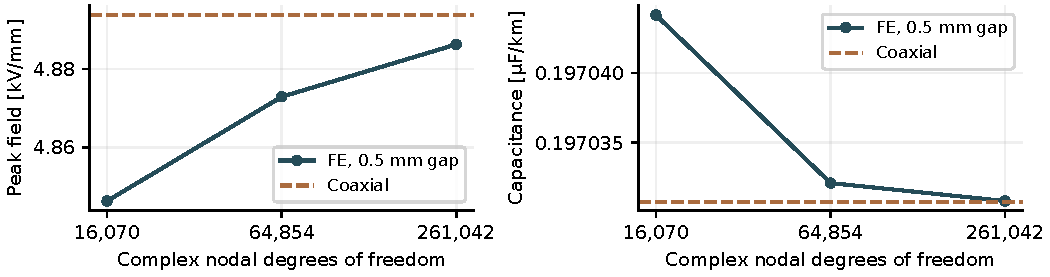
\includegraphics[width=\linewidth]{figures/convergence.pdf}

\codeguide{\setupfile{parameters.pro}: \texttt{MeshFactor};
\setupfile{cable.geo}: Box mesh field; \efile: linear potential space.}
{In Gmsh open \efile. Keep \textbf{Jacket gap [mm]} at 0.5. Set
\textbf{Mesh factor} to 2 and press \textbf{Run}, then repeat at 1 and 0.5.
Save the values before each run overwrites \texttt{res/}. Restore factor 1 afterward.}
{Record ``Dofs'' in the GetDP log, the maximum of \texttt{res/field\_norm.pos}
(V/m), and \texttt{res/capacitance\_uF\_km.dat}. The default factor is 1.}

\newpage
\section*{Q2.4 Healthy-cable stress and a comparison limit}
\assignmentquestion{\QuestionTwoFour}
NKT gives no admissible local electric-field values. We use the external
comparison values of 8 kV/mm RMS at the conductor screen and 4 kV/mm RMS at
the insulation (core) screen from Eskom specification 240-56030625,
Rev.3, \S3.3(i) [Eskom]. That specification applies to 44--132 kV cables;
these are borrowed engineering benchmarks, not an acceptance criterion supplied
for this 33 kV NKT cable.

For concentric ideal screens,
\[
 E_{\rm rms}(r)=\frac{V_{\rm ph,rms}}{r\ln(r_o/r_i)}.
\]
\begin{center}\small
\begin{tabular}{@{}lrr@{}}\toprule
XLPE-side location & Calculated RMS [kV/mm] & Benchmark RMS [kV/mm]\\\midrule
Inner, \(r_i=7.8\) mm & 3.4604 & 8\\
Outer, \(r_o=15.8\) mm & 1.7083 & 4\\\bottomrule
\end{tabular}
\end{center}
The ideal healthy cable is below both benchmarks. This supports the stress
calculation but does not establish dielectric lifetime or certify the cable.
Use the analytical interface values for this comparison: the linear FE gradient
is constant in each triangle and slightly underestimates the boundary maximum.

\codeguide{\efile: \texttt{em} and \texttt{Ele\_Maps};
\setupfile{parameters.pro}: the voltage and XLPE radii.}
{In Gmsh open \efile\ and press \textbf{Run}.}
{\texttt{res/field\_norm.pos} is peak V/m. Divide by \(10^6\sqrt2\) for RMS
kV/mm. \texttt{res/radial\_field\_A.pos} samples 1 \(\mu\)m inside each interface
to avoid ambiguous element lookup exactly on the boundary.}

\section*{Q2.5 Insulation defect}
\assignmentquestion{\QuestionTwoFive}
\pending The current simple geometry contains no defect. A defensible next
case is a circular dry-air void of radius 0.25 mm, centred 8.8 mm from phase A's
axis along \(+x\), with \(\varepsilon_r=1\) and negligible conductivity.
Its nearest edge is 0.75 mm from the inner XLPE interface. These dimensions
and air properties are explicit study assumptions.

In 2D this represents an infinitely long cylindrical channel parallel to the
cable, not a spherical bubble. For a small cylindrical inclusion in an almost
uniform transverse field, the electrostatic estimate is
\(E_{\rm void}/E_{\rm healthy}\simeq2\varepsilon_{\rm XLPE}/
(\varepsilon_{\rm XLPE}+\varepsilon_{\rm air})=1.43\).
This only predicts the tendency to amplify the field; it is not the requested
FE radial-cut comparison. A withstand conclusion also needs a justified gas
breakdown or partial-discharge criterion. Both checks remain to be done.

\codeguide{\setupfile{cable.geo}: add a hole and a separately tagged air surface
in phase-A XLPE. \efile: include that region with its own material law.}
{No defect command exists yet. The Q2.4 command produces only the healthy reference.}
{After implementation, compare the same radial cut for healthy and void cases,
with local mesh refinement around the void. No archived defect result is claimed here.}

\newpage
\section*{Q2.6 Conduction, displacement and conservation}
\assignmentquestion{\QuestionTwoSix}
The implemented peak current densities are
\[
 \hat{\mathbf J}_{c}=\sigma\hat{\mathbf E},\qquad
 \hat{\mathbf J}_{d}=j\omega\varepsilon\hat{\mathbf E},\qquad
 \hat{\mathbf J}=\hat{\mathbf J}_{c}+\hat{\mathbf J}_{d}.
\]
For the analytical maximum field in XLPE at 50 Hz,
\[
 |\hat J_c|=4.89\,10^{-12}~\mathrm{A/m^2},\qquad
 |\hat J_d|=0.03403~\mathrm{A/m^2},\qquad
 \frac{|\hat J_c|}{|\hat J_d|}
 =\frac{\sigma}{\omega\varepsilon}=1.44\,10^{-10}.
\]
The FE maps give approximately \(4.87\,10^{-12}\) and
\(0.03389~\mathrm{A/m^2}\) on the default mesh. Displacement current
overwhelmingly dominates under these material assumptions. The radial charging
current is about \(1.1793~\mathrm{A/km}\) RMS per phase at 33 kV line-to-line;
it must not be confused with the 350 A longitudinal load current.

\textbf{Other materials.} With finite metal conductivity, conduction would
dominate at 50 Hz. The reference semiconducting PE also has conduction-dominated
behaviour; PE and XLPE are primarily dielectric. No current densities in those
other regions are calculated by this XLPE-only model. In particular, a zero or
blank value there cannot establish zero physical current.

\textbf{Conservation: what is checked.} The weak equation enforces
\(\nabla\cdot\hat{\mathbf J}=0\). For the coaxial analytical solution,
\[
 \hat J_r(r)=(\sigma+j\omega\varepsilon)
 \frac{\hat V}{r\ln(r_o/r_i)},\qquad
 2\pi r\hat J_r(r)=\text{constant}.
\]
The total current leaving the inner boundary therefore equals the current
entering the outer boundary. This analytical check is exact.

The current code does not yet export an independent FE boundary-flux balance.
Linear nodal elements do not guarantee pointwise continuous normal current
across every triangle. Thus solving the weak equation is not, by itself, a
quantified conservation test. The remaining check is to integrate total
\(\hat{\mathbf J}\cdot\mathbf n\) on both interfaces and report
\[
 \eta_I=\frac{|I_{\rm inner}+I_{\rm outer}|}
                  {\max(|I_{\rm inner}|,|I_{\rm outer}|)}
\]
using outward normals of the XLPE annulus, then test its mesh dependence.

\codeguide{\efile: \texttt{jCond}, \texttt{jDisp} and their exports in
\texttt{Ele\_Maps}. \setupfile{parameters.pro}: \texttt{sigmaXLPE}, \texttt{epsXLPE}, \texttt{Freq}.}
{In Gmsh open \efile\ and press \textbf{Run}.}
{Open \texttt{res/conduction\_current.pos} and
\texttt{res/displacement\_current.pos}; units are A/m\textsuperscript{2}, peak.
The separate boundary-flux integral is still to be added.}

\newpage
\section*{Q2.7 Capacitance and frequency}
\assignmentquestion{\QuestionTwoSeven}
The coaxial formula from the course Appendix B gives
\[
 C'=\frac{2\pi\varepsilon_0\varepsilon_r}{\ln(r_o/r_i)}
 =1.970307\,10^{-10}~\mathrm{F/m}
 =0.1970307~\mu\mathrm{F/km}.
\]
It assumes concentric circular interfaces, homogeneous linear XLPE, an
infinitely long cable and ideal equipotential semiconductors. Its radii are
the \emph{XLPE interfaces}, 7.8 and 15.8 mm. The semiconductors are excluded
from the dielectric thickness, but their thicknesses determine these radii.

\textbf{FE extraction.} For the three balanced phases, the average per-phase
capacitance is calculated directly from field energy:
\[
 C'_{\rm FE}=\frac{\displaystyle\sum_{k=A,B,C}
 \int_{\Omega_k}\varepsilon|\hat{\mathbf E}|^2\,dA}{3V_p^2}.
\]
The code multiplies F/m by \(10^9\) to export \(\mu\mathrm{F/km}\).
With peak phasors, \(\tfrac14\int\varepsilon|\hat E|^2dA\) is the mean stored
energy. The separately exported \texttt{ElectricEnergy} is twice that mean;
its definition is stated in the source comment so the peak/RMS factor is explicit.

\begin{center}\small
\begin{tabular}{@{}lr@{}}\toprule
Reference & \(C'\) [\(\mu\)F/km per phase]\\\midrule
Coaxial formula & 0.1970307\\
FE, default mesh & 0.1970321\\
FE, fine mesh & 0.1970308\\
NKT maximum & 0.2200000\\\bottomrule
\end{tabular}
\end{center}
The default FE value differs from the analytical value by 0.00069\%.
It is 10.44\% below the NKT maximum. Being below a stated maximum is consistent
with the datasheet, but it is not a match to an exact measured capacitance.
Screen-dimension uncertainty and the borrowed permittivity remain physical uncertainties.

\textbf{Frequency.} Runs at 5, 50, 500 and 5000 Hz on the same gapped mesh all
give \(0.1970321~\mu\mathrm{F/km}\), with unchanged field magnitude to the
shown precision. In each homogeneous annulus, the constant
\(\sigma+j\omega\varepsilon\) cancels from the potential equation.
With imposed voltage and constant properties, this model therefore predicts
frequency-independent capacitance. Real dielectric dispersion, loss tangent
and resistive screens could change that conclusion; none is included here.

\codeguide{\efile: \texttt{CapacitancePerPhase} and its global print.
\setupfile{parameters.pro}: \texttt{Freq}.}
{In Gmsh open \efile. Set \textbf{Frequency [Hz]} to 500 and press \textbf{Run}.
Repeat with 5, 50 and 5000. Restore 50 Hz afterward.}
{Read \texttt{res/capacitance\_uF\_km.dat}: the second column is the real
capacitance. Each run overwrites \texttt{res/}; save the value before the next run.}

\newpage
\section*{Q2.8 Trial improvement: thicker XLPE}
\assignmentquestion{\QuestionTwoEight}
Increase XLPE thickness from 8 to 9 mm, retaining the 7.8 mm inner XLPE radius.
The outer XLPE radius becomes 16.8 mm and the outer semiconductor radius
17.2 mm. In the current parameterisation the copper ring and 43 mm outside
diameter remain fixed. The assumed inner filler shrinks from 1.2 to 0.2 mm.
This is a geometrically feasible trial within our equivalent layers, not a
manufacturer-approved redesign. Its effect on manufacture and heat flow is untested.

\begin{center}\small
\begin{tabular}{@{}lrr@{}}\toprule
Quantity & 8 mm XLPE & 9 mm XLPE\\\midrule
Analytical peak at inner interface [kV/mm] & 4.89372 & 4.50229\\
FE maximum, default mesh factor [kV/mm] & 4.87288 & 4.47403\\
Analytical \(C'\) [\(\mu\)F/km] & 0.197031 & 0.181271\\
FE \(C'\) [\(\mu\)F/km] & 0.197032 & 0.181272\\\bottomrule
\end{tabular}
\end{center}
The analytical maximum falls by 8.00\% and the FE peak by 8.19\%.
Both cases use the 0.5 mm gap and the same 0.25 mm target mesh size.
Capacitance and charging current also decrease by about 8\%.

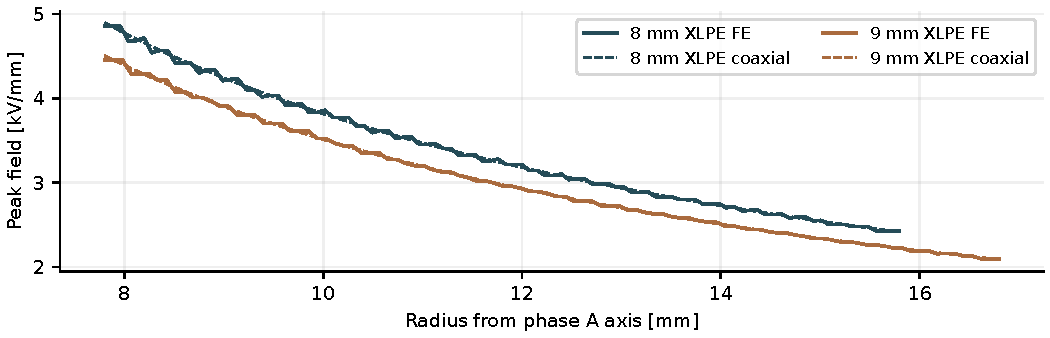
\includegraphics[width=\linewidth]{figures/radial_comparison.pdf}

\codeguide{\setupfile{parameters.pro}: \texttt{tXLPE}, derived radii and fixed
\texttt{rWireIn}. \efile: radial cut and field exports.}
{In Gmsh open \efile. Keep \textbf{Jacket gap [mm]} at 0.5. Set \textbf{XLPE thickness [m]} to \texttt{0.009}
and press \textbf{Run}. The shared ONELAB value is used by both Gmsh and GetDP.}
{Compare \texttt{res/field\_norm.pos},
\texttt{res/radial\_field\_A.pos} and \texttt{res/capacitance\_uF\_km.dat}.
Restore \texttt{0.008} and press \textbf{Run} to return to the baseline.}

\subsection*{Sources and reproducibility}
\small
Geometry and voltage: local \href{../Datasheet 33 kV single core cable XLPE-AL.pdf}{NKT datasheet},
printed pp.19--20. Equations and phasors: local
\href{../NMES_Assignment_2026.pdf}{NMES Assignment 2026}, Appendices A--B.
Material references and their limitations are listed in Section 1, Q1.1.

\textbf{[Eskom]} \refurl{https://www.etenders.gov.za/home/Download/?blobName=b55b97a6-fb2e-492f-8eb0-01bc9574c555.pdf\&downloadedFileName=240-56030625_Specificatin+for+HV+XLPE+cables+and+accessories.pdf}{Specification 240-56030625, Rev.3}, \S3.3(i), Annex B.
Its voltage range differs from our cable; see Q2.4.

Numbers were rerun with Gmsh 4.15.2 and GetDP 4.0.0-git-259f4c38.
For convergence, \texttt{MeshFactor} was 2, 1 and 0.5; other inputs stayed at
their defaults. Regenerated triangle/node counts can vary slightly with the
Gmsh version and triangulation. In ONELAB, changing \textbf{Output > Directory}
to \texttt{results/case-name} preserves that run's maps.

If Gmsh requests the GetDP executable, choose
\path{ONELAB Software/Gmsh.app/Contents/MacOS/getdp} in the course folder beside
this repository. Search \texttt{Q2.1}, \texttt{Q2.3}, etc. in the source to find
the blocks used by each answer. The electric-folder \texttt{cable.geo} contains
only an include of the shared geometry, so there is one geometry definition.
\end{document}
